
\begin{frame}
	\frametitle{Direct forces calculation}
	
	Acceleration of particle $i$:
	\begin{align*}
		\ddot{\mathbf{r}}_i = - G \sum\limits_{j=1}^{N}  \frac{m_j}{[(\mathbf{r}_i - \mathbf{r}_j)^2 + \epsilon^2 ]^{\frac{3}{2}}} (\mathbf{r}_i - \mathbf{r}_j)
	\end{align*}

$\epsilon$ is the \textit{softening length}. It's purposes are:
\begin{itemize}
	\item computational efficiency
	\item avoid large angle scatterings
	\item avoid expense to calculate orbits in a singular potential
	\item prevent the possibility of formation of bound particle pairs
\end{itemize}
	
\end{frame}






\begin{frame}
	\frametitle{Direct force calculation results for varying softening}
	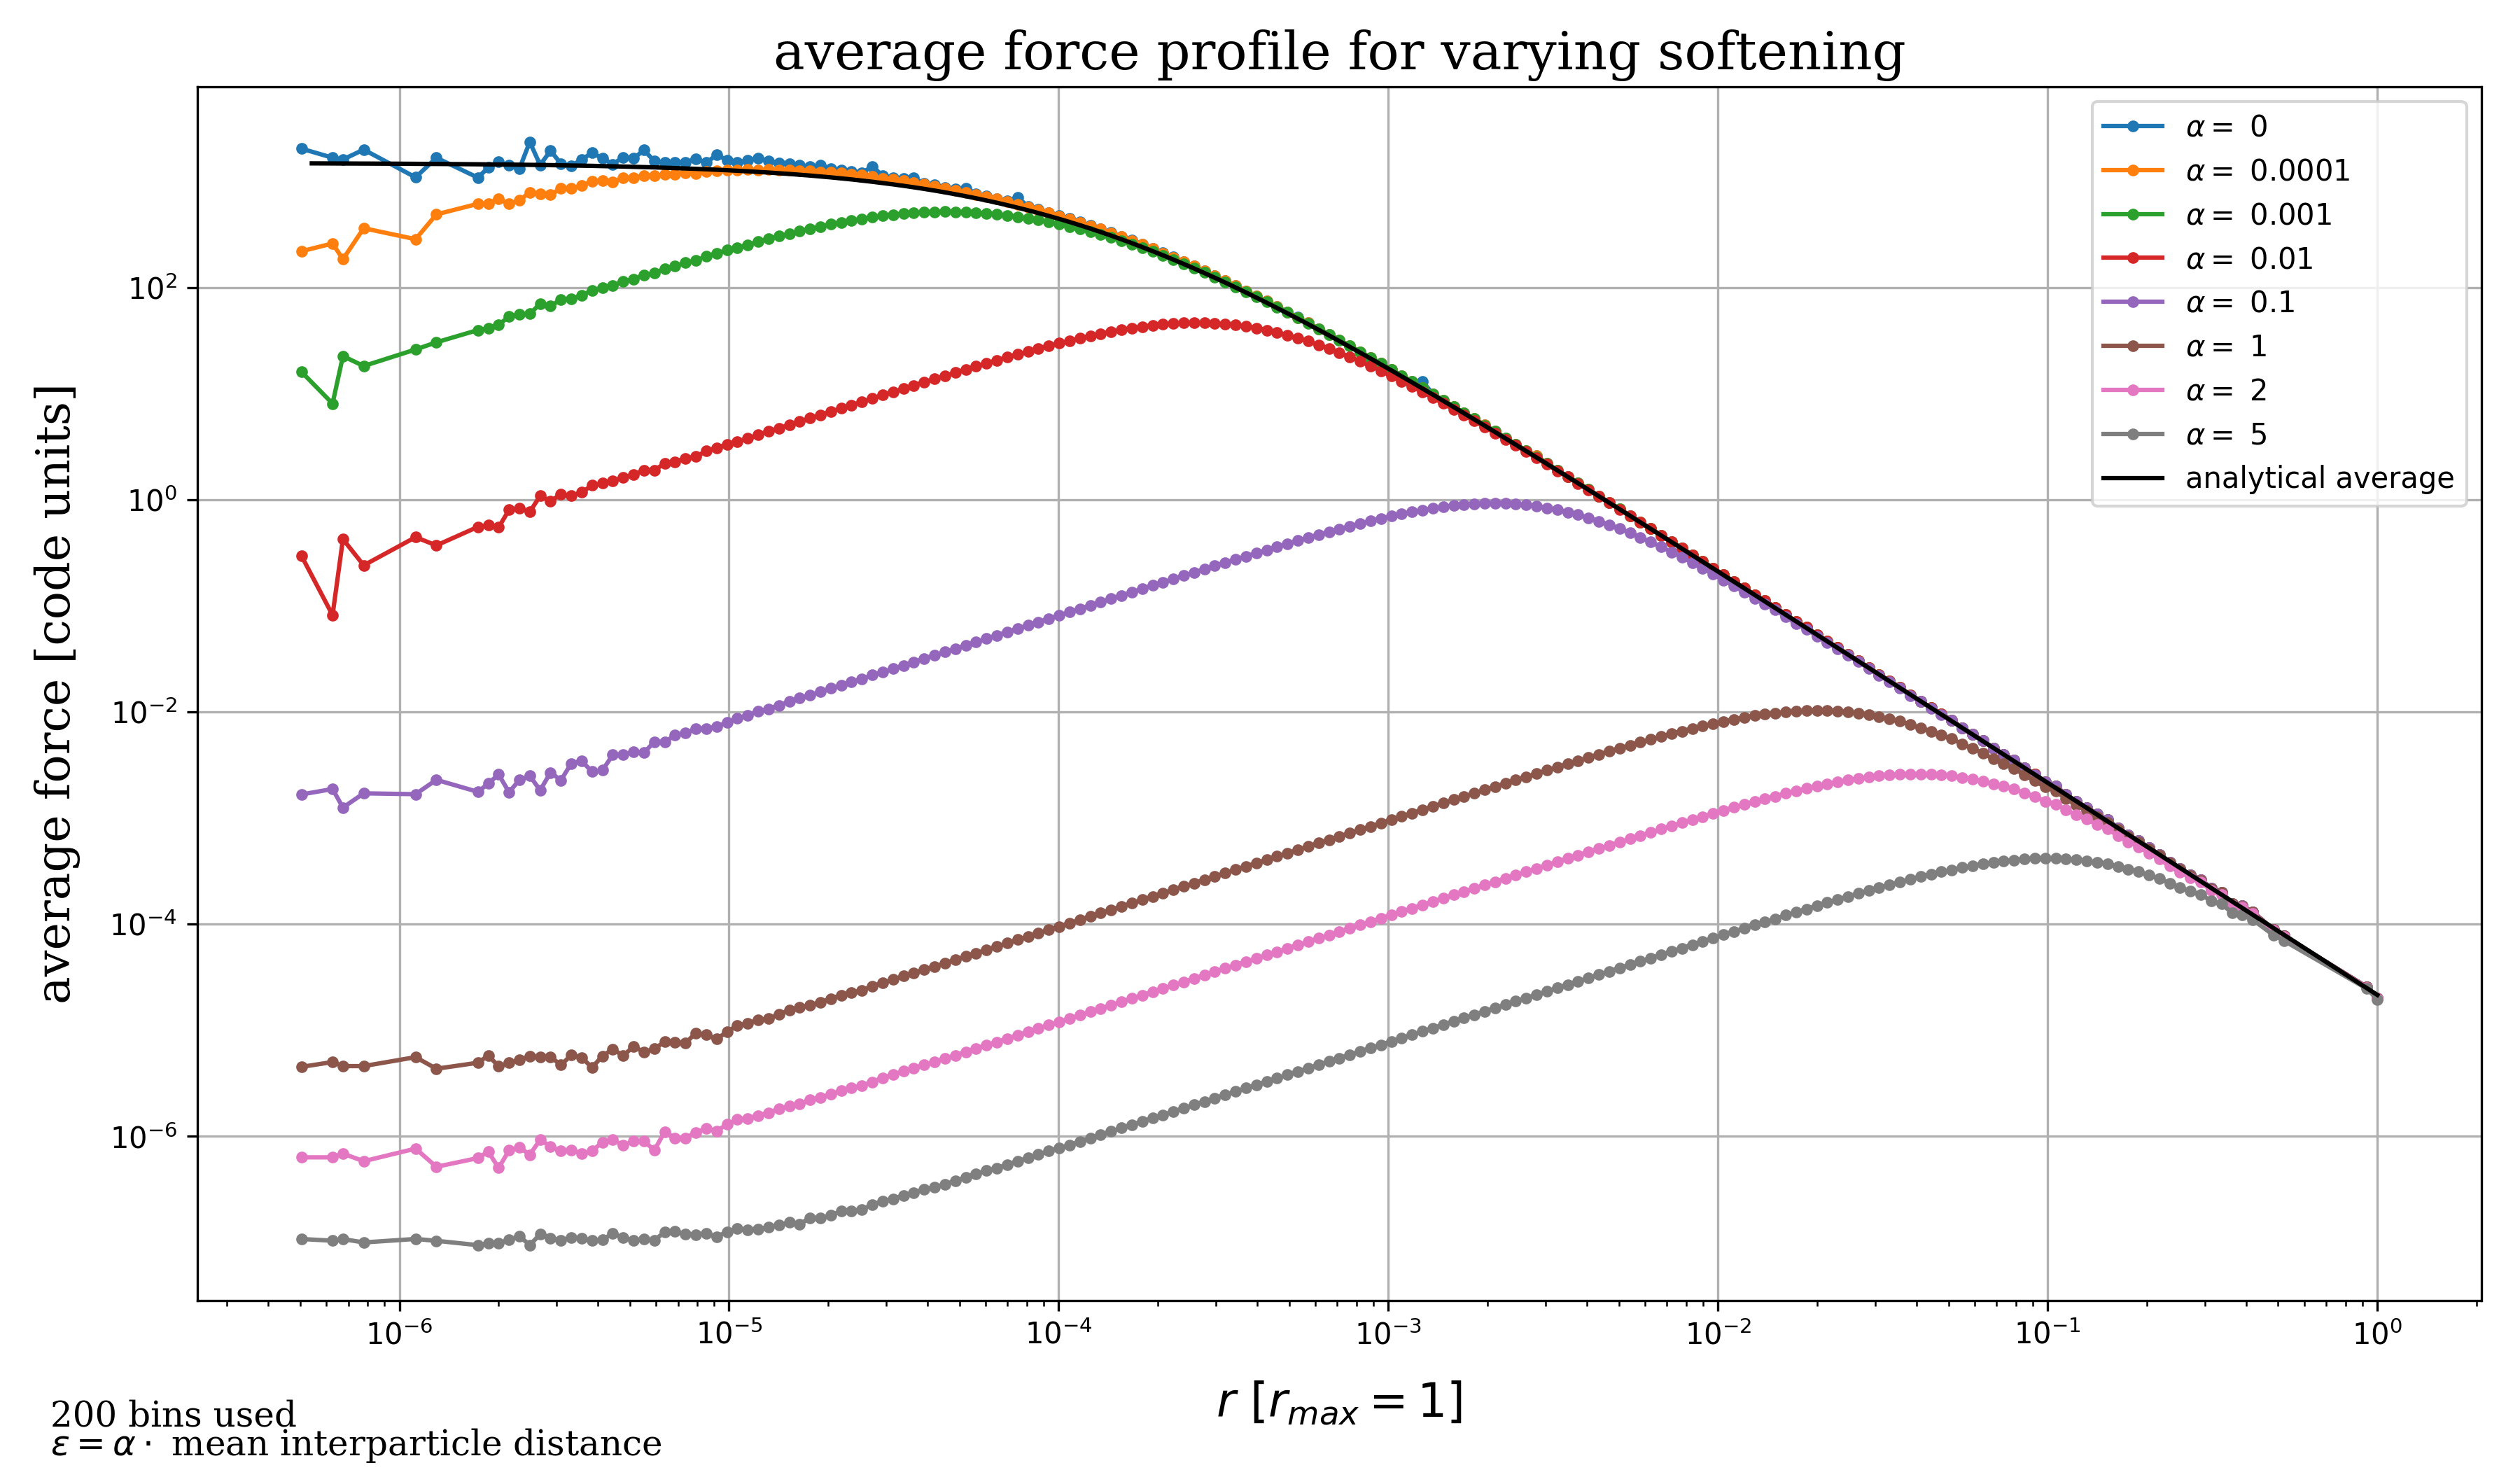
\includegraphics[width=\textwidth]{../results/average_direct_force/average_force_plot.png}
\end{frame}
